% Options for packages loaded elsewhere
\PassOptionsToPackage{unicode}{hyperref}
\PassOptionsToPackage{hyphens}{url}
%
\documentclass[
]{book}
\usepackage{amsmath,amssymb}
\usepackage{iftex}
\ifPDFTeX
  \usepackage[T1]{fontenc}
  \usepackage[utf8]{inputenc}
  \usepackage{textcomp} % provide euro and other symbols
\else % if luatex or xetex
  \usepackage{unicode-math} % this also loads fontspec
  \defaultfontfeatures{Scale=MatchLowercase}
  \defaultfontfeatures[\rmfamily]{Ligatures=TeX,Scale=1}
\fi
\usepackage{lmodern}
\ifPDFTeX\else
  % xetex/luatex font selection
\fi
% Use upquote if available, for straight quotes in verbatim environments
\IfFileExists{upquote.sty}{\usepackage{upquote}}{}
\IfFileExists{microtype.sty}{% use microtype if available
  \usepackage[]{microtype}
  \UseMicrotypeSet[protrusion]{basicmath} % disable protrusion for tt fonts
}{}
\makeatletter
\@ifundefined{KOMAClassName}{% if non-KOMA class
  \IfFileExists{parskip.sty}{%
    \usepackage{parskip}
  }{% else
    \setlength{\parindent}{0pt}
    \setlength{\parskip}{6pt plus 2pt minus 1pt}}
}{% if KOMA class
  \KOMAoptions{parskip=half}}
\makeatother
\usepackage{xcolor}
\usepackage{longtable,booktabs,array}
\usepackage{calc} % for calculating minipage widths
% Correct order of tables after \paragraph or \subparagraph
\usepackage{etoolbox}
\makeatletter
\patchcmd\longtable{\par}{\if@noskipsec\mbox{}\fi\par}{}{}
\makeatother
% Allow footnotes in longtable head/foot
\IfFileExists{footnotehyper.sty}{\usepackage{footnotehyper}}{\usepackage{footnote}}
\makesavenoteenv{longtable}
\usepackage{graphicx}
\makeatletter
\def\maxwidth{\ifdim\Gin@nat@width>\linewidth\linewidth\else\Gin@nat@width\fi}
\def\maxheight{\ifdim\Gin@nat@height>\textheight\textheight\else\Gin@nat@height\fi}
\makeatother
% Scale images if necessary, so that they will not overflow the page
% margins by default, and it is still possible to overwrite the defaults
% using explicit options in \includegraphics[width, height, ...]{}
\setkeys{Gin}{width=\maxwidth,height=\maxheight,keepaspectratio}
% Set default figure placement to htbp
\makeatletter
\def\fps@figure{htbp}
\makeatother
\setlength{\emergencystretch}{3em} % prevent overfull lines
\providecommand{\tightlist}{%
  \setlength{\itemsep}{0pt}\setlength{\parskip}{0pt}}
\setcounter{secnumdepth}{5}
\usepackage{booktabs}
\ifLuaTeX
  \usepackage{selnolig}  % disable illegal ligatures
\fi
\usepackage[]{natbib}
\bibliographystyle{plainnat}
\IfFileExists{bookmark.sty}{\usepackage{bookmark}}{\usepackage{hyperref}}
\IfFileExists{xurl.sty}{\usepackage{xurl}}{} % add URL line breaks if available
\urlstyle{same}
\hypersetup{
  pdftitle={LPS 30 Discussion Notes},
  pdfauthor={Ryan Chen},
  hidelinks,
  pdfcreator={LaTeX via pandoc}}

\title{LPS 30 Discussion Notes}
\author{Ryan Chen}
\date{2024-02-29}

\begin{document}
\maketitle

{
\setcounter{tocdepth}{1}
\tableofcontents
}
\hypertarget{about}{%
\chapter{About}\label{about}}

These are notes for Ryan Chen's LPS 30 Discussion Sections (Monday 1-2 p.m. and 4-5 p.m.). These notes summarize the material covered in discussion. For this course, it primarily consists of definitions, exercises and worked out solutions to exercises. These notes are intended for students who want to review course material and students which miss discussion for whatever reason. They are not a replacement for attending discussion section.

\hypertarget{propositions-and-validity}{%
\chapter{Propositions and Validity}\label{propositions-and-validity}}

{[}I have tried to include as much detail as possible in this week's notes. This is because we did not have discussion in week 2, and so this is meant to be a sort of replacement. Future weeks may be more sparse.{]}

\hypertarget{propositions}{%
\section{Propositions}\label{propositions}}

What is a proposition? According to the slides, \emph{a proposition is a thing we could believe or disbelieve}. Importantly, propositions are expressed by sentences (propositions are not sentences themselves). More importantly, propositions are expressed by a certain kind of sentence: declarative sentences. So, the question of identifying which sentences express propositions is really a question of identifying the declarative sentences.

There are a number of ways to test whether or not a sentence is a declarative sentence. Here, is one given in lecture: (Step One) take the sentence you want to test and stick ``I believe that\ldots{}'' in front of it. (Step Two) If the result of sticking ``I believe that\ldots{}'' in front of the sentence still makes sense, then the original sentence expresses a proposition.

\textbf{{[}Example One{]}} Consider the sentence ``It is raining''. (Step One) To test this sentence, I stick ``I believe that\ldots{}'' in front of it. So, I get, ``I believe that it is raining''. (Step Two) Now, I ask myself, does it make sense to say ``I believe that it is raining''? It does. Therefore, ``It is raining'' expresses a proposition.

\textbf{{[}Example Two{]}} Consider the sentence ``Coffee is tasty''. (Step One) To test this sentence, I stick ``I believe that\ldots{}'' in front of it. So, I get, ``I believe that coffee is tasty''. (Step Two) Now, I ask myself, does it make sense to say ``I believe that coffee is tasty''? It does. Therefore, ``Coffee is tasty'' expresses a proposition. (Note: most people think that whether or not coffee is tasty is a matter of personal preference. Nonetheless, the sentence ``coffee is tasty'' still expresses a proposition. Just because a sentence expresses a proposition the truth (or falsity) of which depends on one's own taste, does not mean that that sentence does not express a proposition.)

\textbf{{[}Example Three{]}} Consider the sentence ``Please close the door''. (Step One) To test this sentence, I stick ``I believe that\ldots{}'' in front of it. So, I get, ``I believe that please close the door''. (Step Two) Now, I ask myself, does it make sense to say ``I believe that please close the door''. It does not. Therefore, ``Please close the door'' does not express a proposition.

From now on, I will be less wordy on these examples:

\textbf{{[}Example Four{]}} Consider the sentence ``Earth is the eighth planet in the solar system''. (Step One) ``I believe that Earth is the eighth planet in the solar system''. (Step Two) Does this make sense? Yes. Therefore, ``Earth is the eighth planet in the solar system'' expresses a proposition. (Note: Earth is of course not the eighth planet in the solar system. Nonetheless, ``Earth is the eighth planet in the solar system'' expresses a proposition. Just because a sentence is false does not mean it does not express a proposition.)

\textbf{{[}Example Five{]}} Consider the sentence ``I believe that it will rain tomorrow''. (Step One) ``I believe that I believe that it will rain tomorrow''. (Step Two) Does this make sense? Yeah (If this is not obvious to you, replace the original sentence with ``John believes that it will remain tomorrow''; it should be clear to you that ``I believe that John believes that it will remain tomorrow'' makes sense to say. Now the original example should sound better).

Now that we know what a proposition is, we can define what an argument is. \emph{An argument is a list of propositions}. We call the last proposition, the \emph{conclusion} of the argument. We call all the other propositions, the \emph{premises}.

\hypertarget{validity}{%
\section{Validity}\label{validity}}

We want to know which arguments are good arguments. To do so, we use the notion of validity. \emph{An argument is valid if and only if if the premises are true then the conclusion must be true}. I prefer this alternative, but equivalent definition: \emph{An argument is valid if and only if it is impossible for the premises to be true and the conclusion false}.

The definition tells us how to assess whether or not an argument is valid or not. (Step One) First, we \emph{suppose} that the premises of the argument are true. Note that this does not mean that the premises are in fact true. You suppose that the premises are true for the sake of argument. (Step Two) Now you ask, whether or not the conclusion \emph{must} be true given the supposition that you make in step one (i.e., under the (potentially) hypothetical situation where the premises are true).

\textbf{{[}Example One{]}} Consider the argument:

\begin{enumerate}
\def\labelenumi{\arabic{enumi}.}
\tightlist
\item
  All cats are dogs.
\item
  All dogs are books.
\item
  Therefore, all cats are books.
\end{enumerate}

(Step One) Let us suppose that all cats are dogs and all dogs are books. That is, we are under the hypothetical situation in which all cats are dogs and all dogs are books (never mind what such a universe would look like, just suppose they are true!). (Step Two) Under such a supposition, does it \emph{necessarily} follow that all cats are books? Yes! For now, I hope you share my intuition on this matter; as the course progress, we will develop more and more tools to help you see why this conclusion necessarily follows. (Note: we are starting this course with propositional logic. It turns out that in propositional logic, there is no obvious way to represent the argument just given as valid. So look forward to predicate logic where we can represent such arguments)

\textbf{{[}Example Two{]}} Consider the argument:

\begin{enumerate}
\def\labelenumi{\arabic{enumi}.}
\tightlist
\item
  If Ryan is writing these notes at 2 am then Ryan will wake up tired in the morning.
\item
  If Ryan will wake up tired in the morning then Ryan will get coffee in the morning.
\item
  Ryan is writing these notes at 2 am.
\item
  Therefore, Ryan will get coffee in the morning.
\end{enumerate}

(Step One) Let us suppose that all the premises are true. (Step Two) Since premise three tells us that Ryan is writing these notes at 2 am then when we combine that fact with premise one, it seems that we must conclude that Ryan will wake up tired in the morning. Well, since Ryan will wake up tired in the morning, then we can combine that fact with premise two, and we must conclude that Ryan will get coffee in the morning. This shows that the argument is valid. Here, I tried to use a bit of reasoning to show you why you must arrive at the conclusion.

\textbf{{[}Example Three{]}} Consider the argument:

\begin{enumerate}
\def\labelenumi{\arabic{enumi}.}
\tightlist
\item
  If Ryan is mortal then Ryan will one day pass away.
\item
  Ryan is mortal.
\item
  Therefore, Ryan is a PhD student
\end{enumerate}

(Step One) Let us suppose that all the premises are true. (Step Two) You should ask yourself, can it be the case that premise 1 and 2 are true while premise 3 false? It certainly seems so. I could have not pursued graduate school and pursued some other career. Nothing about the premises seems to necessitate the conclusion that Ryan is a PhD student. Hence, the argument is invalid (Note: the premises and the conclusion of this argument are true, yet the argument is invalid. There is a general lesson here. Just because an argument has true premises and a true conclusion does not mean that it is valid)

From now on, I will skip writing out step one.

\textbf{{[}Example Four{]}} Consider the argument:

\begin{enumerate}
\def\labelenumi{\arabic{enumi}.}
\tightlist
\item
  Ryan prefers cats to dogs.
\item
  If water is H2O then copper conducts electricity.
\item
  Copper does not conduct electricity.
\item
  Therefore, water is not H2O.
\end{enumerate}

(Step Two) Since, by premise 3, Copper does not conduct electricity, it cannot be the case that water is H2O. Why? Here's a bit of reasoning: If water was H2O then by premise 2 I would be forced to conclude that copper conducts electrity. By premise 3, it is not the case that copper conducts electricity. Well it cannot be the case that copper conducts electricity and it does not conduct electricity; that is just absurd! We have to think to ourselves, is there a way that both premise 2 and premise 3 are true concurrently? Yes! it must then be the case that water is not H2O. Now I am not forced to conclude that copper conducts electricity and so all the premises can remain true at the same time. Therefore, the argument is valid. (Note: notice here that premise 1 is never used. All that is needed to get the conclusion are premises 2 and 3. This tells us something important: an argument may have irrelevant premises and still be valid)

\textbf{{[}Example Five{]}} Consider the argument:

\begin{enumerate}
\def\labelenumi{\arabic{enumi}.}
\tightlist
\item
  Squirtle ate food at 4 pm four days ago.
\item
  Squirtle ate food at 4 pm three days ago.
\item
  Squirtle ate food at 4 pm two days ago.
\item
  Squirtle ate food at 4 pm yesterday.
\item
  Therefore, Squirtle will eat food at 4 pm today.
\end{enumerate}

(Step Two) Can it be the case that even if I accept all the premises, the conclusion is false? Yes! Squirtle might be stopped from eating food at 4 pm; maybe, Squirtle just is not hungry. Hence, this argument is invalid. (Note: notice that there is still something compelling about this argument. This sort of argument is called an inductive argument, and while invalid, they seem to be used all the time. Saying why such arguments are good has been a major problem for philosophers for centuries).

\textbf{{[}Example Six{]}} Consider the argument:

\begin{enumerate}
\def\labelenumi{\arabic{enumi}.}
\tightlist
\item
  Tom went to the mall and Jerry followed after Tom.
\item
  Therefore, Jerry followed after Tom.
\end{enumerate}

(Step Two) If Tom went to the mall and Jerry followed after Tom is true then it simply just followed that Jerry followed after Tom! Hence, this argument is valid.

\textbf{{[}Example Seven{]}} Consider the argument:

\begin{enumerate}
\def\labelenumi{\arabic{enumi}.}
\tightlist
\item
  Either it is the case that Tom went to the mall or Jerry went to the mall.
\item
  Therefore, Tom went to the mall.
\end{enumerate}

(Step Two) Well, just because we suppose that either Tom went to the mall or Jerry went to the mall does not mean that it must follow that Tom went to the mall. It could be the case that Jerry went to the mall and Tom did not go to the mall. Under that possibility, premise 1 would still be true but the conclusion would be false. Therefore, the argument is invalid.

\textbf{{[}Example Eight{]}} Consider the argument:

\begin{enumerate}
\def\labelenumi{\arabic{enumi}.}
\tightlist
\item
  If it is raining then everyone wins the lottery.
\item
  Everyone wins the lottery.
\item
  Therefore, it is raining.
\end{enumerate}

(Step Two) Well, just because everyone won the lottery does not mean that it is raining. What premise 1 tells us is that if it is raining then we must conclude that everyone wins the lottery. But it does not tell us that it is in fact the case that it is raining. It is perfectly possible for it to be sunny and clear out and everyone wins the lottery. In which case, all the premises are true and the conclusion false. Therefore, the argument is invalid.

Next week, we will return to a couple more arguments.

\hypertarget{soundness}{%
\section{Soundness}\label{soundness}}

\emph{An argument is sound if and only if it is valid and the premises are actually true}. Notice the difference between soundness and validity. Validity requires that \textbf{if} the premises are true then the conclusion must be true. That is, it requires that under the hypothetical situation that the premises are true then the conclusion must be true. Soundness requires that the premises are in fact true.

I will not say more about soundness here. Of course, you are welcome to ask questions in discussion or office hours. I think it is beneficial to sit down and think through the differences between the definitions of validity and soundness and the relations that they bear to one another (your homework makes you think about this).

\hypertarget{argument-forms}{%
\section{Argument Forms}\label{argument-forms}}

To get an argument form, you look at a given argument, look for sentences which express propositions in them and replace those sentences with letters like \(A,B,C,\ldots\). Note that you are allowed to replace parts of sentences which express propositions with letters as well.

\textbf{{[}Example One{]}} Consider the argument:

\begin{enumerate}
\def\labelenumi{\arabic{enumi}.}
\tightlist
\item
  Either the world is round or the sun is round.
\item
  If the world is round then the sea is wet.
\item
  The sun is round.
\item
  Therefore, the world is round.
\end{enumerate}

Notice that in premise 1, the sentence ``either the world is round or the sun is round'' has two parts ``the world is round'' and ``the sun is round'' which themselves express propositions. Hence, we can represent this premise as ``Either \(A\) or \(B\)'' where \(A\)=the world is round and \(B\)=the sun is round. Again, in premise 2, the sentence ``If the world is round then the sea is wet'' has two parts ``the world is round'' and ``the sea is wet'' which express propositions. We can represent this premise with ``if \(A\) then \(C\)'' where it continues to be the case that \(A\)=the world is round and \(C\)=the sea is wet. The other two premises are straightforward and we get:

\begin{enumerate}
\def\labelenumi{\arabic{enumi}.}
\tightlist
\item
  Either \(A\) or \(B\)
\item
  If \(A\) then \(C\)
\item
  \(B\)
\item
  Therefore, \(A\)
\end{enumerate}

Some argument forms are valid. They are not valid in the same sense that an argument is valid. Instead, \emph{an argument form is valid if and only if every instance of that argument form is valid}.

That is, when we are given an argument form we are given something that looks like an argument but with a bunch of letters like \(A,B,C,D,E,\ldots\) (just see the previous example). To get an instance of that argument form, you replace all these letters with sentences (which express propositions). So, continuing with our example:

\begin{enumerate}
\def\labelenumi{\arabic{enumi}.}
\tightlist
\item
  Either \(A\) or \(B\)
\item
  If \(A\) then \(C\)
\item
  \(B\)
\item
  Therefore, \(A\)
\end{enumerate}

We see that there are three letters \(A\), \(B\), and \(C\) which appear in that argument form. To get an instance of this form, let \(A\)=Tom is funny, let \(B\)=Tom is hungry, and let \(C\)=Jerry is tired (these are just random sentences that I have chosen). Then putting these sentences into the argument form yields:

\begin{enumerate}
\def\labelenumi{\arabic{enumi}.}
\tightlist
\item
  Either Tom is funny or Tom is hungry.
\item
  If Tom is funny then Jerry is tired.
\item
  Tom is hungry.
\item
  Therefore, Tom is funny.
\end{enumerate}

I leave it to you to verify that this argument is in fact invalid. Since, the argument form has an instance which is invalid, the argument form itself is invalid.

What is an example of a valid argument form? Here are two examples:

\textbf{{[}Example One{]}} Consider the argument form:

\begin{enumerate}
\def\labelenumi{\arabic{enumi}.}
\tightlist
\item
  If \(A\) then \(B\)
\item
  \(A\)
\item
  Therefore, \(B\)
\end{enumerate}

\textbf{{[}Example Two{]}} Consider the argument form:

\begin{enumerate}
\def\labelenumi{\arabic{enumi}.}
\tightlist
\item
  \(A\) and \(B\)
\item
  Therefore, \(B\)
\end{enumerate}

How do we check? At this point in this course we do not have the means to verify that all instances of this argument form are valid. The problem is that to check whether or not an argument form is valid, we need to answer the following question: if I substitute in any sentences (which express propositions) for \(A\) and \(B\), then is the resulting argument valid? The crucial bit here is that you need to check for \emph{any} sentence and there are an infinite number of possible sentences in English which express propositions. It would take you an awfully long time to go through an infinite number of sentences.

Thankfully, checking for invalid argument forms is doable. Here is another example (now with explicity steps):

\textbf{{[}Example Three{]}} Consider the argument form:

\begin{enumerate}
\def\labelenumi{\arabic{enumi}.}
\tightlist
\item
  \(A\)
\item
  If \(C\) then \(A\) and \(B\)
\item
  Therefore, \(C\)
\end{enumerate}

To check that this is an invalid argument form you need to come up with sentences (which express propositions) such that if you substitute those sentences in, the resulting argument is invalid. So, (Step One), come up with as many sentences as there are different letters in the argument form. Here there are three letters, \(A\), \(B\) and \(C\), so we need three sentences. Let us use: \(A\)=``Bob is funny'', \(B\)=``Jerry is silly'', and \(C\)=``It is hot out today''. Next, (Step Two), we need to substitute these into the argument form:

\begin{enumerate}
\def\labelenumi{\arabic{enumi}.}
\tightlist
\item
  Bob is funny.
\item
  If it is hot out today then Bob is funny and Jerry is silly.
\item
  Therefore, it is hot out today.
\end{enumerate}

Now, (Step Three), check for validity. So, now you need to follow the steps to check for validity. Hopefully, at this point you can check that this argument is invalid.

\hypertarget{translation}{%
\chapter{Translation}\label{translation}}

This week in discussion we mainly practiced translation problems. There are a couple key skills to learn here:

\begin{enumerate}
\def\labelenumi{\arabic{enumi}.}
\tightlist
\item
  Given a English sentence which expresses a proposition, you should be able to translate it into propositional logic.
\item
  Given an argument, you should be able to translate it into propositional logic.
\item
  Given a string of symbols, you should be able to evaluate whether or not it is a formula in propositional logic.
\item
  Given a formula in propositional logic, you should be able to translate it back into English.
\end{enumerate}

We only practiced the first skill in discussion. The second skill should follow immediately from knowing how to do the first. We will touch more on the third skill in week 4, but also see the Translation and Language Slides on canvas, starting from slide 25. Finally, skill 4 was not covered, so I will give an example of this at the end of these notes.

\hypertarget{translating-from-english-to-propositional-logic}{%
\section{Translating from English to Propositional Logic}\label{translating-from-english-to-propositional-logic}}

In a question where you are asked to translate an English sentence or an argument into propositional logic, you do the following:

\begin{itemize}
\tightlist
\item
  (Step One) Provide a dictionary. That is, for every part of a sentence that expresses a proposition in the sentence, assign it a unique lower-case letter. {[}NOTE: Sometimes this involves first rewriting the sentence, so that it is clear what all the sentence parts are. More on this in the example{]}
\item
  (Step Two) Go through that sentence and replace all the parts of the sentence with their corresponding letters according to the dictionary.
\item
  (Step Three) Go through the result of step two and examine all the English expressions which remain. If any of the left-over expressions correspond to a propositional connective, then look for the propositional letters which the connective is binding together. Then, following the rules for constructing formulas in propositional logic, replace the expression, with the symbol corresponding to the propositional connective.
\end{itemize}

Note that these steps give you the general strategy that you should use when translating. Sometimes, you may need to still bring your intuitions to the table when doing this sort of exercise.

{[}Example One{]} Consider the sentence: ``If Tom went to the mall then Jerry fell down the stairs''. (Step One) We see here that ``Tom went to the mall'' and ``Jerry fell down the stairs'' are sentences which express propositions. These are the parts of the larger sentence ``If Tom went to the mall then Jerry fell down the stairs'' which we want to assign unique letters. So, let \(t\)=Tom went to the mall and \(j\)=Jerry fell down the stairs. (Step Two) When we replace the parts of the sentences with the propositional letters, we get ``If \(t\) then \(j\)''. (Step Three) Now, we see that the phrase is of the form ``If\(\ldots\) then\(\ldots\)'' which corresponds to the propositional connective \(\supset\). We also note that the conditional is operating on \(t\) and \(j\) with \(t\) being the antecedent and \(j\) being the consequent. Hence, following the rules for how to build formulas in propositional logic, we get \((t \supset j)\).

{[}Example Two{]} Consider the sentence: ``Tom and Jerry went to the mall''. (Step One) Here, we can first rewrite the sentence to reveal its underlying structure. ``Tom and Jerry went to the mall'' can be rewritten as ``Tom went to the mall and Jerry went to the mall'' (this trick does not always work). Now, we can provide a dictionary: \(t\)=Tom went to the mall, \(j\)=Jerry went to the mall. (Step Two) Replacing the sentences with their propositional letters, we get ``\(t\) and \(j\)''. (Step Three) We note that this is of the form ``\(\ldots\)and\(\ldots\)'' and that it binds together, \(t\) and \(j\), so we get \((t \& j)\).

{[}Example Three{]} I go a bit quicker in this example. Consider the sentence: ``If Tom went to the mall and Jerry went to the mall then Adam went to the mall''. (Step One) Dictionary: \(t\)=Tom went to the mall, \(j\)=Jerry went to the mall, and \(a\)=Adam went to the mall. (Step Two) Replacing the sentences with their propositional letters, we get ``If \(t\) and \(j\) then \(a\)''. (Step Three) Now here is where we need to be a bit careful.We need to note that the ``If\(\ldots\)then\(\ldots\)'' clause has as its antecedent ``\(t\) and \(j\)'' and its consequent \(a\).''\(t\) and \(j\)'' just translates into \((t \& j)\) (see Example Two). So, we end up with ``If \((t \& j)\) then \(a\)''. This just translates into \(((t \& j) \supset a)\) (see Example One).

\hypertarget{practice-problems}{%
\section{Practice Problems}\label{practice-problems}}

Here are the questions in section (A) and section (B) which we worked on in discussion section. If you have not tried doing them, I recommend trying to translate them before looking at the solutions:

\begin{itemize}
\tightlist
\item
  (A1) If Mary is the sister of Jane then Jane is Bill's aunt.
\item
  (A2) Either Jones bluffed his hand or Jones is crazy.
\item
  (A3) Neither Jones nor Sally were happy with the colour blue.
\item
  (A4) Tables are solid if and only if books are readable.
\item
  (A5) Tom went to the mall and Jerry went to bed.
\item
  (A6) Tom went to the mall but Jerry went to bed.
\item
  (A7) If Jesse lies and Frank cheats then the Thagard's are crooks.
\item
  (A8) If Jesse lies then if Frank cheats then the Thagard's are crooks.
\item
  (A9) If Jesse and Frank are crooks then either George is a crook or the sky is falling.
\item
  (B1) If Alfred is a spy then Rudolf is breaking the law.
\item
  (B2) Alfred is a spy only if Rudolf is breaking the law.
\item
  (B3) Alfred is a spy if Rudolf is breaking the law.
\item
  (B4) Alfred is a spy unless Rudolf is breaking the law.
\item
  (B5) It will be hot out tomorrow and quite damp, unless the eastern winds pick up today.
\item
  (B6) Debra will not leave until the others do, but, only if Meredith is in the office.
\item
  (B7) If the ball is red then Ash won the competition unless the second ball drawn is blue.
\item
  (B8) If Lee wants it, Lee can get it, but Lee should not blame Sarah if Sarah gets in trouble.
\item
  (B9) If Justin's heart stops beating then Justin will live if the doctors apply electric shock.
\end{itemize}

\hypertarget{practice-problem-solutions}{%
\section{Practice Problem Solutions}\label{practice-problem-solutions}}

Here are the solutions. If it is obvious, then I leave the dictionary out:

\begin{itemize}
\tightlist
\item
  (A1) \((m \supset j)\)
\item
  (A2) Dictionary: \(j\)=Jones bluffed his hand, \(c\)=Jones is crazy. Answer: \((j \lor c)\)
\item
  (A3) \(\sim(j \lor s)\) (it is equally acceptable to write \((\sim j \& \sim s)\))
\item
  (A4) \((t \equiv b)\)
\item
  (A5) \((t \& j)\)
\item
  (A6) \((t \& j)\) {[}NOTE: A5 and A6 have the same answer{]}
\item
  (A7) \(((j \& f) \supset t)\)
\item
  (A8) \((j \supset (f \supset t))\)
\item
  (A9) \(((j \& f) \supset (g \lor s))\)
\item
  (B1) \((a \supset r)\)
\item
  (B2) \((a \supset r)\) {[}NOTE: B1 and B2 have the same answer{]}
\item
  (B3) \((r \supset a)\)
\item
  (B4) \((\sim r\supset a)\)
\item
  (B5) \((\sim e \supset (h \& d))\)
\item
  (B6) This one is trickier than I thought and so I won't provde an answer here. You won't get a question this tricky.
\item
  (B7) Here are two possible answers: \((\sim b \supset (r \supset a))\) and \((r \supset (\sim b \supset a))\)
\item
  (B8) Dictionary: \(w\)=Lee wants it, \(g\)=Lee gets it, \(b\)=Lee should blame Sarah, \(t\)=Sarah gets in trouble. Answer: \(((w \supset g) \& (t \supset \sim b))\)
\item
  (B9) \((h \supset (e \supset l))\)
\end{itemize}

\hypertarget{translating-from-propositional-logic-to-english}{%
\section{Translating from Propositional Logic to English}\label{translating-from-propositional-logic-to-english}}

{[}Example{]} Consider the following dictionary \(a\)=Albert is funny, \(b\)=Bart is smart, and \(c\)=Cassandra is athletic. Then consider the following formula \((\sim a \supset (b \& c))\). To translate this back into English, let us first translate the connectives back into English. Let us start with the \(\supset\), so we get ``If \(\sim a\) then \((b \& c)\)''. Now we translate the \(\sim\) to get, ``If it is not the case that \(a\) then \((b \& c)\)''. Next is the \(\&\) to get, ``If it is not the case that \(a\) then \(b\) and \(c\)''. Finally, we plug the sentences back in: ``If it is not the case that Albert is funny then Bart is smart and Cassandra is athletic''. Sometimes, if you follow this sort of procedure, if does not make sense. You may have to move words around in order to make it make sense.

\hypertarget{truth-tables}{%
\chapter{Truth Tables}\label{truth-tables}}

\hypertarget{how-to-fill-out-a-truth-table}{%
\section{How to Fill Out a Truth Table}\label{how-to-fill-out-a-truth-table}}

You may be asked to provide and fill out the truth table for a given formula. In what follows, I provide steps as to how to do this. Note that I do this in a painstakingly detailed way. Your answers do not have go step-by-step in the way I have outlined here; just the final truth table is fine. In any case, make sure you understand why I take each step that I take.

\begin{enumerate}
\def\labelenumi{\arabic{enumi}.}
\item
  First, look at the formula and identify the distinct propositional letters in the formula. Knowing how many propositional letters there are and which ones there are will tell you how to fill out the left-hand side of your table. For example, if you have the formula \(((p \supset q) \lor (q \lor \sim p))\) then there are only two distinct propositional letters \(p\) and \(q\). If you have the formula \(((q \lor j) \& (j \equiv r))\), there are three distinct propositional letters \(q\), \(j\), and \(r\).
\item
  With the propositional letters you have identified in step 1., you will start the left hand side of your truth table with those letters. You will then put the formula you want to do the truth table for to the right of those letters. So, suppose that you have a formula \((p \supset (q \supset p))\) with letters \(p\) and \(q\), you will start it as follows:
\end{enumerate}

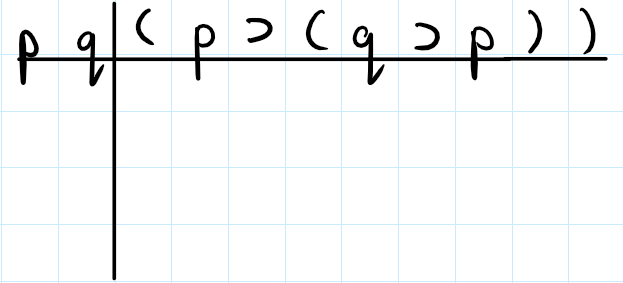
\includegraphics{Pictures/Week4Picture1.png}
If instead, you have the formula \(((r \lor w) \& (\sim j \supset u))\), then you will start your table as follows:

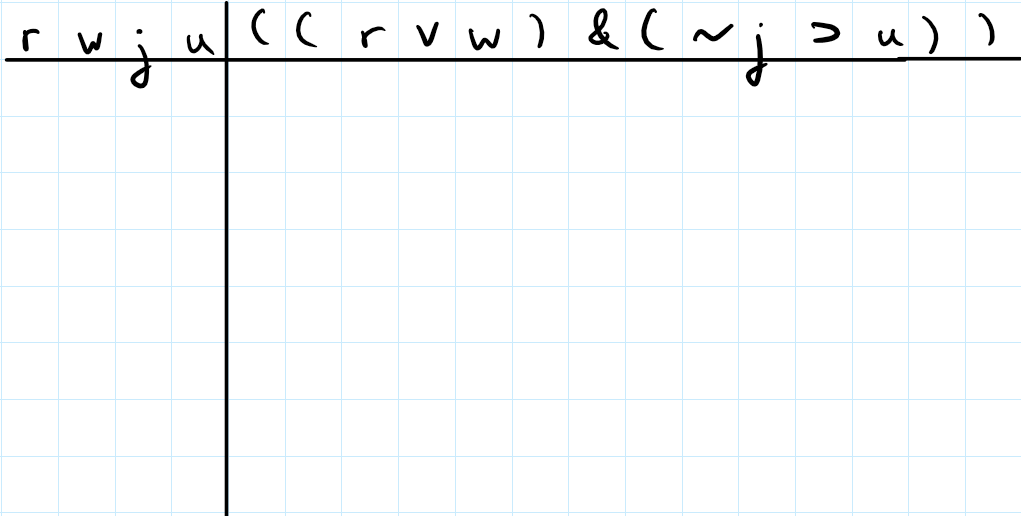
\includegraphics{Pictures/Week4Picture2.png}
3. Next, you fill out the columns for the propositional letters on the left hand side. To do this, you follow a pattern.

First, you determine the number of rows that you need to fill out. For \(n\) different propositional letters, you will have \(2^n\) rows. For example, if you have \(2\) propositional letters, then you will have \(2^2 = 4\) rows. If you have \(3\) propositional letters, then you will have \(2^3 = 8\) rows.

Secondly, starting from the right most propositional letter, you fill out the column by alternating 0s and 1s for each row (this is where figuring out how many rows there are comes in handy; for example, if you know that there will be \(8\) rows, then you will alternate until you have filled out all \(8\) rows). Then you move to the propositional letter one column to the left and you alternate 00 and 11 down the column (you will stop here if you only have two propositional letters). Here is an example:

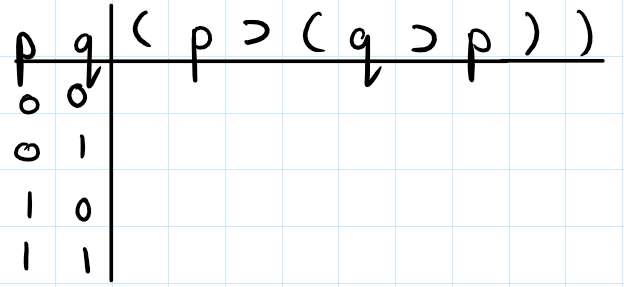
\includegraphics{Pictures/Week4Picture3.png}

If you have more than two propositional letters, move one column to the left and you alternate 0000 and 1111 down the column (you will stop here if you only have three propositional letters). Here is an example:

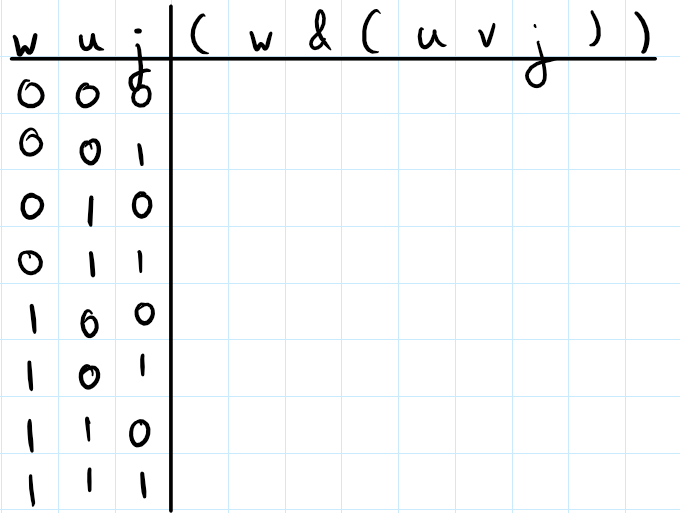
\includegraphics{Pictures/Week4Picture4.png}

If you have more than three propositional letters, then move one column to the left and you alternate 00000000 and 11111111 down the column (you will stop here if you only have four propositional letters). I leave it to you to continue the pattern.

\begin{enumerate}
\def\labelenumi{\arabic{enumi}.}
\setcounter{enumi}{3}
\tightlist
\item
  Now, you can start filling out the columns under the formula that you are concerned with. My advice is to just fill out whatever columns you \emph{can} fill out. This will require you to know how the formulas compose together to form bigger formulas. Here is an example (slightly different from the one I covered in person, in discussion): consider the formula \((p \lor j) \& (\sim p \supset \sim (j \equiv p))\). We start off the table as follows:
\end{enumerate}

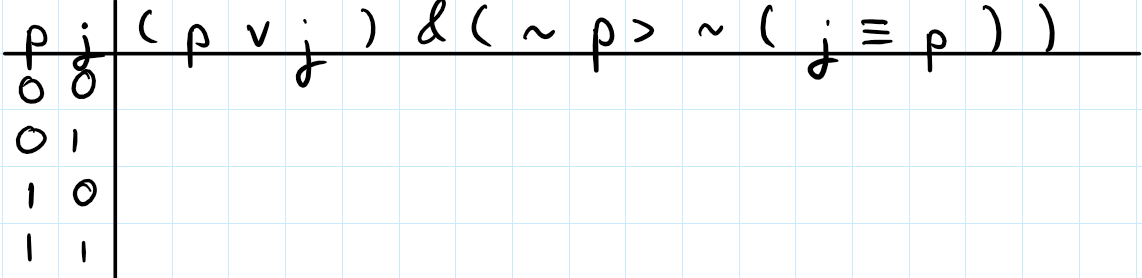
\includegraphics{Pictures/Week4Picture5.png}
Now, we look at the propositional connectives and see which ones we can start to evaluate. Let us consider the \(\&\) connective. Can we evaluate that one yet? Well, we could only evaluate the \(\&\) if we knew the truth value columns of the two formulas that it binds. In this case, the \(\&\) binds together the \((p \lor j)\) and the \((\sim p \supset \sim (j \equiv p))\). Do we currently know what the truth value columns for those formulas are? No.~The truth value column of \((p\lor j)\) would be the column under the \(\lor\) as the \(\lor\) binds together the \(p\) and the \(j\) to create \((p \lor j)\). Can we figure it out? Yes, since we already have the truth value columns for \(p\) and \(j\):

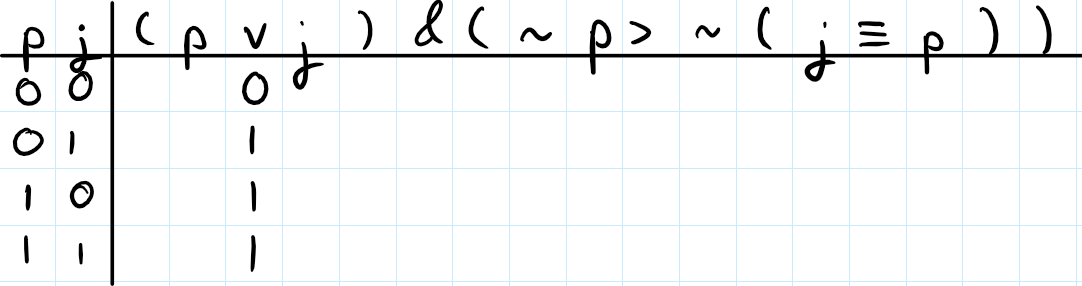
\includegraphics{Pictures/Week4Picture6.png}
So, the left conjunct of the \(\&\) is taken care of. We now need to find the truth value column of the right conjunct. In this case, the column is the one under the \(\supset\) symbol. This is because to form \((\sim p \supset \sim (j \equiv p))\), the \(\supset\) symbol binds together the \(\sim p\) and the \(\sim (j \equiv p)\) formulas. Do we have the truth values of \(\sim p\) and \(\sim (j \equiv p)\)? No.~Can we figure it out? Well, we can quickly fill out the \(\sim p\) since we know the truth value column of \(p\):

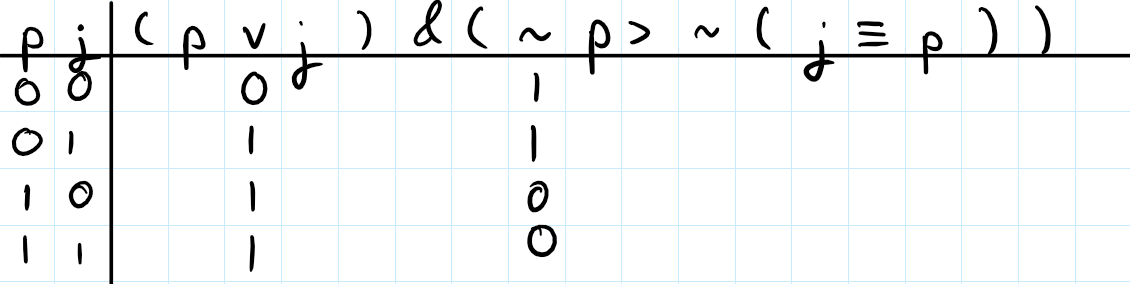
\includegraphics{Pictures/Week4Picture7.png}

Can we do this for \(\sim (j \equiv p)\)? No.~To determine the truth value column under the \(\sim\), we need to first know the truth value column under the \(\equiv\) in \((j \equiv p)\). Thankfully, we can find that since we already have the truth values of \(j\) and \(p\):

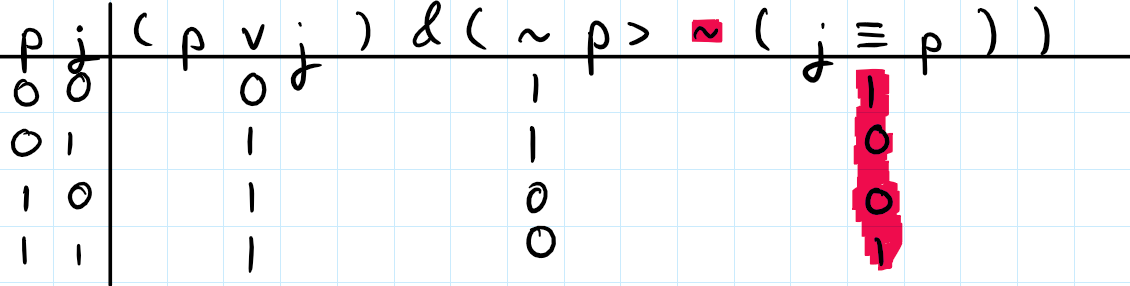
\includegraphics{Pictures/Week4Picture8.png}

Now, we can figure out the truth value column under the \(\sim\). I have highlighted in magenta-red(?), the column that the negation \(\sim\) operates over:

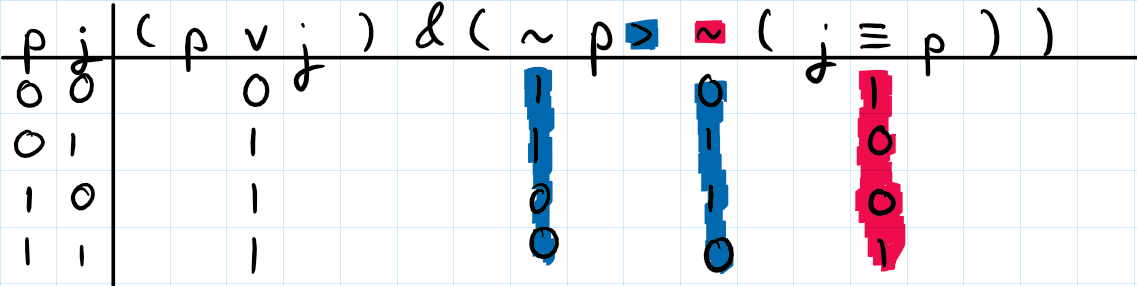
\includegraphics{Pictures/Week4Picture9.png}

Now, remember that the \(\supset\) binded together the \(\sim p\) formula and the \(\sim (j \equiv p)\). The blue highlighted columns are the truth value columns for those formulas and we have both of them now. So we can evaluate the conditional:

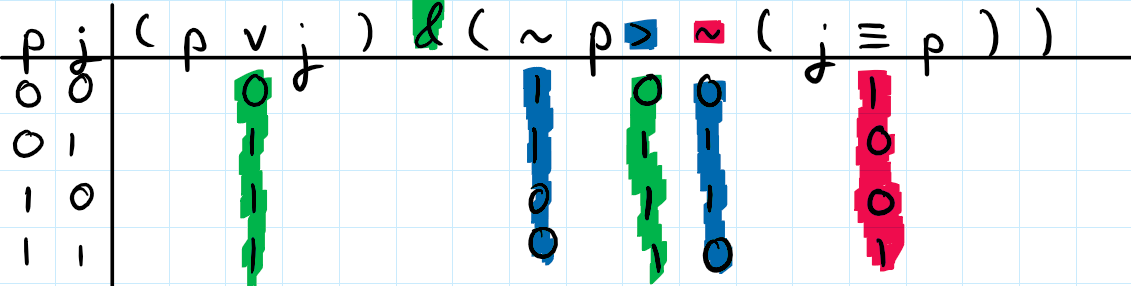
\includegraphics{Pictures/Week4Picture10.png}

Finally, remember that the \(\&\) binded together the \((p \lor j)\) formula and the \((\sim p \supset \sim (j \equiv p))\) formula. The highlighted green columns are the truth value columns for those two formulas. Hence, we can now evaluate the \(\&\), which I will highlight in yellow:

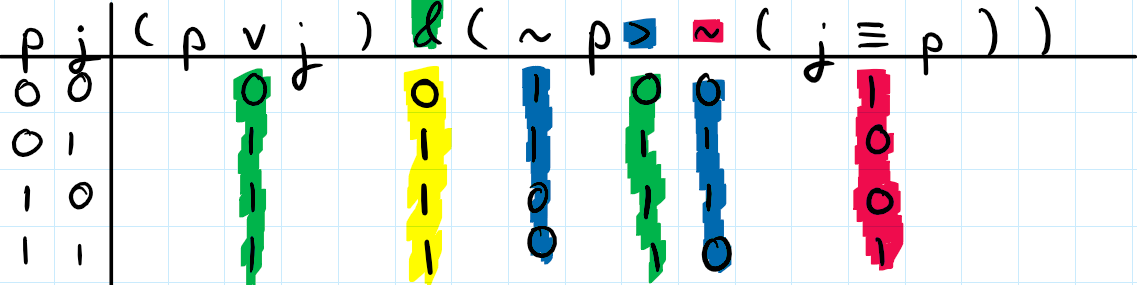
\includegraphics{Pictures/Week4Picture11.png}

That yellow column is the truth value column for the entire formula.

\hypertarget{definitions-of-tautology-contradiction-and-contingency}{%
\section{Definitions of Tautology, Contradiction and Contingency}\label{definitions-of-tautology-contradiction-and-contingency}}

The concepts of tautology, contradiction, and contingency are really important in logic. Sometimes, just by looking at a formula you may be able to tell whether or not it is a tautology, contradiction or contingency, but sometimes you will not be able to. Thankfully, truth tables are one way to always tell whether or not a formula is one of these three.

So, given a formula, to ascertain whether or not it is a tautology, contradiction or a contingency, you:

\begin{enumerate}
\def\labelenumi{\arabic{enumi}.}
\tightlist
\item
  Fill out its truth table.
\item
  Look at the truth value column for the formula that you are concerned with. If the column is all 1s then it is a \emph{tautology}. If the column is all 0s then its a \emph{contradiction}. If the column includes at least one 1 and at least one 0 then it is a \emph{contingency}.
\end{enumerate}

That is all there is to it. Informally, a tautology is a formula which is always true; a contradiction is a formula which is always false; and a contingency is a formula which is sometimes true and sometimes false.

\hypertarget{checking-validity-of-arguments-with-a-truth-table}{%
\section{Checking Validity of Arguments with a Truth Table}\label{checking-validity-of-arguments-with-a-truth-table}}

Sometimes you will be asked to check the validity of an argument using a truth table. The question will often look like ``is \(\phi_1,\phi_2,\ldots,\phi_n \therefore \psi\) valid?'' (the \(\phi_1,\phi_2,\ldots,\phi_n,\psi\) just stand for arbitrary formulas). The formulas before the \(\therefore\) are the premises and the formula after the \(\therefore\) is the conclusion. The procedure for answering such questions is an extension of how to fill out the truth table of a given formula:

\begin{enumerate}
\def\labelenumi{\arabic{enumi}.}
\tightlist
\item
  First look across all the formulas \(\phi_1,\phi_2,\ldots,\phi_n, \psi\) and look at all the distinct propositional letters in those formulas. Start off the left hand side of your truth table with those propositional letters (this is just like the first step for ``How to Fill out a Truth Table''; the only exception is now you are looking at letters across multiple formulas). Next, put the premises \(\phi_1,\ldots,\phi_n,\psi\) to the right of the propositional letters with a line in between each of them. You will end up with something looking like:
\end{enumerate}

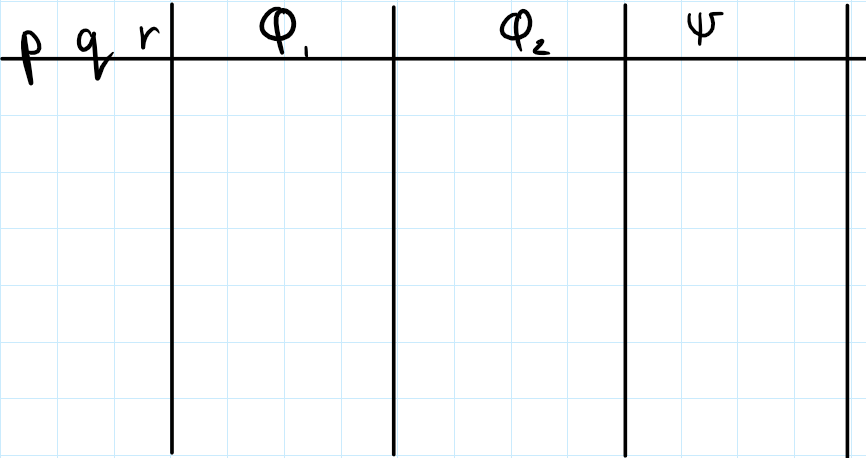
\includegraphics{Pictures/Week4Picture12.png}
(This is a case with two premises \(\phi_1\), \(\phi_2\) and the conclusion \(\psi\)). Next, you fill out the columns for the propositional letters on the left-hand side of the table as you would normally (as in, do the same as step 3. for ``How to Fill Out a Truth Table'').

\begin{enumerate}
\def\labelenumi{\arabic{enumi}.}
\setcounter{enumi}{1}
\item
  Then, working with only one formula at a time, fill out the truth table. For example, if you are working on \(\phi_1\), then you just fill out that truth table; you do not need to consider the other formulas at all. You should end up with truth value columns for all of the formulas (i.e., the premises and the conclusion).
\item
  To evaluate validity, start from the top row and see whether or not it is a row in which the truth value of every premise is a 1. If it is a row in which all the premises are 1, then check whether or not the conclusion is also a 1. If it is \emph{not}, then the argument is invalid and you can stop checking. If it is a 1 then you move onto the row below and repeat the checking procedure. If there is no row below, then you are done and the argument is valid.
\end{enumerate}

\hypertarget{practice-problems-1}{%
\section{Practice Problems}\label{practice-problems-1}}

Provide the truth table for the following (I omit A3, since it is too easy):

\begin{itemize}
\tightlist
\item
  (A1) \((p \lor q) \lor r\)
\item
  (A2) \(\sim (p \& q)\)
\item
  (A4) \((\sim p \lor \sim q)\)
\item
  (A5) \(((p \supset q) \equiv (\sim p \lor q))\)
\end{itemize}

Is the following formula a tautology, contradiction or a contingency? Use a truth table to evaluate:

\begin{itemize}
\tightlist
\item
  (B1) \((p \supset p)\)
\item
  (B2) \((p \supset \sim\sim p)\)
\item
  (B3) \((p \& q) \lor (q \& p)\)
\item
  (B4) \(\sim (p \supset (q \supset p))\)
\item
  (B5) \(((q \supset p) \supset (\sim q \supset \sim p))\)
\item
  (B6) \(((p \supset ((p \supset q) \equiv (p \& \sim r))) \lor r)\)
\end{itemize}

Which of the following arguments are valid?

\begin{itemize}
\tightlist
\item
  (C1) \((\sim p \lor q), q \therefore \sim p\)
\item
  (C2) \((\sim p \supset (q \lor p)), \sim p \therefore q\)
\item
  (C3) \((p \equiv (q \& \sim p)), (q\supset p) \therefore (q \lor p)\)
\end{itemize}

\hypertarget{solutions}{%
\section{Solutions}\label{solutions}}

Under the main column you should have (left-to-right = top-to-bottom)

\begin{itemize}
\tightlist
\item
  (A1) \(01111111\)
\item
  (A2) \(1110\)
\item
  (A4) \(1110\)
\item
  (A5) \(1111\)
\end{itemize}

Then for the other questions, I just give the answers you should arrive at (I also quickly did these so there is a possibility of a mistake):

\begin{itemize}
\tightlist
\item
  (B1) Tautology
\item
  (B2) Tautology
\item
  (B3) Contingency
\item
  (B4) Contradiction
\item
  (B5) Contingency
\item
  (B6) Contingency
\item
  (C1) Invalid
\item
  (C2) Valid
\item
  (C3) Invalid
\end{itemize}

\hypertarget{propositional-logic-trees}{%
\chapter{Propositional Logic Trees}\label{propositional-logic-trees}}

\hypertarget{satisfiability}{%
\section{Satisfiability}\label{satisfiability}}

{[}Definition{]} A collection of formulas \(\{A_1,A_2,\ldots,A_n\}\) is satisfiable just in case there there is some row of the truth table (we also call a row on the truth table, an evaluation) where \(A_1,A_2,\ldots,A_n\) are all true.

Why does this matter for us? Because trees are a method for determining whether or not a collection of formulas is satisfiable. And it is because of their ability to determine satisfiability, that trees are also a method for determining the validity of arguments. Here's how (keep track of the italicized phrases in the following list; they indicate which phrases change):

\begin{enumerate}
\def\labelenumi{\arabic{enumi}.}
\tightlist
\item
  Recall the definition of validity. An argument is valid just in case it is impossible for all the premises to be true and the conclusion to be false.
\item
  And 1. is equivalent to saying: An argument is \emph{invalid} just in case it is \emph{possible} for all the premises to be true and the conclusion false.
\item
  And 2. is equivalent to saying: An argument is invalid just in case it is possible for all the premises to be true and the \emph{negation} of the conclusion to be true
\item
  And 3. is equivalent to saying: An argument is invalid just in case the premises and the negation of the conclusion are satisfiable.
\end{enumerate}

And so, suppose that we have some method for determining whether or not any collection of formulas is satisfiable. Then whenever we are given some argument, we can find out whether or not that argument is valid by using that method to determine whether or not the premises and the negation of the conclusion are satisfiable.

\hypertarget{trees}{%
\section{Trees}\label{trees}}

Trees tell us whether or not a collection of formulas is satisfiable. In this course, there are three main kinds of questions which we can use trees to answer:

\begin{itemize}
\tightlist
\item
  Is \(A_1,\ldots,A_n\) satisfiable?
\item
  Is \(A\) a tautology, contradiction, or a contingency?
\item
  Is \(A_1,\ldots,A_n \therefore B\) valid?
\end{itemize}

To be able to use the tree method, you will need to be able to identify the main connective of a formula. Again, the main connective is the last connective used to construct the formula that you are concerned with. The main connective always has a tree rule associated with it. And so once you have identified the main connective, then you know immediately, which tree rule to apply (there is an exception with the negation symbol). There are only three cases in which you can no longer apply a tree rule: (i) you have already applied a tree rule to that formula; (ii) the formula is an atomic formula (aka, a propositional letter); (iii) the formula is a negated atomif formula (aka, a propositional letter with a single negation in front of it).

For example, in \((((p \supset q) \lor j) \& k)\) the main connective is \(\&\). This is because the only way to construct \((((p \supset q) \lor j) \& k)\) (in accordance with the rules for making formulas) is to take \(((p \supset q) \lor j)\) and \(k\) and concatenate them together with the \(\&\) symbol in between (and with parentheses at the ends). Because the \(\&\) symbol is the main connective, the tree rule you can apply to \((((p \supset q) \lor j) \& k)\) is the \(\&\) rule {[}Look to the slides or your own notes to recall what this rule looks like{]}.

I mentioned earlier that negation has an exception. It has an exception because when the negation \(\sim\) symbol as the main connective (and it is not just a negated atomic), you have to look at the formula without the negation to determine which tree rule to use. For example, in \(\sim (q \supset p)\) the \(\sim\) is the main connective. Now you should ignore the \(\sim\), so we get \((q \supset p)\) whose main connective is the \(\supset\). This tells you to use the negated conditional rule {[}NOTE: you do not use the conditional rule here; it is the \emph{negated conditional rule}{]}.

I will not cover the other aspects of how to do the trees here. You have to review on your own: how to start the tree, when you can close a branch, how to extend the tree out, and strategies for which formulas to do first.

{[}How to Answer Questions About Satisfiability{]} Suppose that you are asked whether or not \(A_1,\ldots,A_n\) is satisfiable. Then:

\begin{enumerate}
\def\labelenumi{\arabic{enumi}.}
\tightlist
\item
  Start your tree with \(A_1,\ldots,A_n\)
\item
  Apply tree rules until you obtain a complete tree.
\item
  If there is at least one open branch on the tree, then \(A_1,\ldots,A_n\) is satisfiable. Otherwise, the tree is complete and closed and hence \(A_1,\ldots,A_n\) is unsatisfiable.
\end{enumerate}

{[}How to Answer Questions About Tautology, Contingency, and Contradiction{]} Suppose that you are asked whether or not \(A\) is a tautology, contingency, or a contradiction. Then:

\begin{enumerate}
\def\labelenumi{\arabic{enumi}.}
\tightlist
\item
  Start a tree with \(A\)
\item
  Apply tree rules until you obtain a complete tree.
\item
  If the tree is complete and closed, then \(A\) is a contradiction {[}Why? Because if the tree is complete and closed (with \(A\) as its start), this means \(A\) is unsatisfiable which means it is never true; to be a contradiction just is to be never true{]}. Otherwise, the tree has at least one open branch and continue to step 4
\item
  Start a tree with \(\sim A\)
\item
  Apply tree rules until you obtain a complete tree.
\item
  If the tree is complete and closed, then \(A\) is a tautology {[}Why? Because if the tree is complete and closed (with \(\sim A\) as its start), this means that \(\sim A\) is unsatisfiable. This means that \(\sim A\) is never true which implies that \(A\) is always true; to be a tautology is just to always be true{]}. If the tree has at least one open branch, then it is neither a contradiction nor a tautology, and hence, must be a contingency.
\end{enumerate}

{[}How to Answer a Question About the Validity of an Argument{]} Suppose you are asked whether or not \(A_1,\ldots,A_n \therefore B\) is a valid argument. Then:

\begin{enumerate}
\def\labelenumi{\arabic{enumi}.}
\tightlist
\item
  Start your tree with \(A_1,\ldots,A_n\) and \(\sim B\)
\item
  Apply tree rules until you obtain a complete tree.
\item
  If the tree is complete and closed the argument is valid. Otherwise, the complete tree has at least one open branch and is invalid.
\item
  If you are asked to provide a counter example evaluation (you can only do this if the argument is invalid) then you pick any open branch and identify when atomic formulas or negated atomic formulas appear on that branch. If an atomic formula appears on that branch, then give it an assignment of \(1\) on a row in the truth table. If the negated atomic appears on the branch, then give it an assignment of \(0\) on that same row. If a propositional letter does not appear on the branch, but it is in at least one of the formulas in the argument, then you can give it any truth value.
\end{enumerate}

\hypertarget{soundness-and-validity}{%
\section{Soundness and Validity}\label{soundness-and-validity}}

Note that we write:
\[
A_1,\ldots,A_n \vdash B
\]
to mean that the tree that starts with \(A_1,\ldots,A_n, \sim B\) closes. This means that \(A_1,\ldots,A_n, \sim B\) is not satisfiable which is equivalent to saying that \(A_1,\ldots,A_n \therefore B\) is valid. Remember, that we write:
\[
A_1,\ldots,A_n \vDash B
\]
for when the argument \(A_1,\ldots,A_n \therefore B\) is valid. Hence, for propositional logic, the following theorem is true:

Soundness
\[
        \text{If } A_1,\ldots, A_n \vdash B \text{ then } A_1,\ldots, A_n \vDash B
\]
which has its counterpart:

Completeness
\[
        \text{If } A_1,\ldots, A_n \vDash B \text{ then } A_1,\ldots, A_n \vdash B
\]
What is the difference between the two? Soundness tells us that our tree process never misleads us. If the tree with \(A_1,\ldots,A_n, \sim B\) closes then there is no row on the truth table with premises \(A_1,\ldots,A_n, B\) such that the premises are true and the conclusion false. But notice the antecedent of the preceding statement: ``if the tree with \(A_1,\ldots,A_n,\sim B\) closes'\,'. Suppose that \(A_1,\ldots,A_n, \sim B\) is unsatisfiable (equivalently, that the argument \(A_1,\ldots,A_n \therefore B\) is valid). We would like it to be the case that the tree starting with \(A_1,\ldots,A_n,\sim B\) does close, but the Soundness property does not guarantee that it will close. It is the Completeness Theorem which tells us we do not need to worry about this; if \(A_1,\ldots,A_n, \sim B\) is unsatisfiable then the tree will close.

\hypertarget{practice-problems-2}{%
\section{Practice Problems}\label{practice-problems-2}}

\begin{itemize}
\tightlist
\item
  (A1) Is \(((k \& (t \& j)) \supset \sim \sim (j \equiv \sim (\sim t \lor k))\) satisfiable?
\item
  (A2) Is \(\{(p \supset (j \lor z)), \sim (j \lor z), p\}\) satisfiable?
\item
  (A3) Is \(\{((q \lor j) \supset z), ((\sim z \& u) \equiv (o \lor k)), (q \& k)\}\) satisfiable?
\item
  (B1) Is \(\sim ((\sim p \& \sim j) \equiv (p \lor j))\) a tautology, contradiction or contingency?
\item
  (B2) Is \(((f \supset h) \& \sim(\sim f \lor h))\) a tautology, contradiction or contingency?
\item
  (C1) Is the argument \(d, (a \supset b), (e \supset c), (\sim a \supset (d \supset e)), ((b \lor c) \supset f), \therefore f\) a validity?
\item
  (C2) Is the argument \((\sim q \lor \sim j),(k \& f), (f \supset (\sim j \lor k)), (k \supset (\sim q \lor j)) \therefore (j \lor k)\) a validity?
\item
  (C3) Is the argument \((((a \lor b) \& (c \lor d)) \supset k), \sim(\sim a \lor \sim d), (c \equiv \sim b), \sim (b \supset d) \therefore k\) a validity?
\end{itemize}

\hypertarget{solutions-1}{%
\section{Solutions}\label{solutions-1}}

\begin{itemize}
\tightlist
\item
  (A1) Satisfiable
\item
  (A2) Unsatisfiable
\item
  (A3) Unsatisfiable
\item
  (B1) Tautology
\item
  (B2) Contradiction
\item
  (C1) Valid
\item
  (C2) Valid
\item
  (C3) Valid
\end{itemize}

\hypertarget{predicate-logic-overview}{%
\chapter{Predicate Logic Overview}\label{predicate-logic-overview}}

In this short document, I will overview what we have done in propositional logic and how that will transfer over to predicate logic. {[}Note: I do not cover the Sorites Paradox in discussion. It is examinable material; if you have questions about it, email me or come see me in office hours{]}.

\hypertarget{language}{%
\section{Language}\label{language}}

We began propositional logic with translations from English into the language of propositional logic. The language of propositional logic just consists of:

\begin{enumerate}
\def\labelenumi{\arabic{enumi}.}
\tightlist
\item
  Propositional letters \(p,q,r,\ldots\)
\item
  Propositional connectives \(\sim, \&, \lor, \supset, \equiv\)
\item
  Parentheses \((,)\)
\end{enumerate}

Predicate logic adds four new kinds of symbols to the language and gets rid of propositional letters. We end up with:

\begin{enumerate}
\def\labelenumi{\arabic{enumi}.}
\tightlist
\item
  Names (or Constants) \(a,b,c\)
\item
  Predicates \(A,B,C\)
\item
  Variables \(x,y,z\)
\item
  Quantifiers \(\forall, \exists\)
\item
  Propositional connectives \(\sim, \&, \lor, \supset, \equiv\)
\item
  Parentheses \((,)\)
\end{enumerate}

\hypertarget{syntax}{%
\section{Syntax}\label{syntax}}

Soon after doing translation work, we gave a syntax for propositional logic. A syntax is just a set of rules for determining when a string of symbols (i.e., symbols put next to one another) counts as a \emph{formula}. Recall, that the syntax for propositional logic is given by:

\begin{enumerate}
\def\labelenumi{\arabic{enumi}.}
\tightlist
\item
  All propositional letters are formulas.
\item
  If \(A\) and \(B\) are formulas then \(\sim(A)\), \((A \& B)\), \((A \lor B)\), \((A \supset B)\), \((A \equiv B)\).
\item
  Nothing else is a formula.
\end{enumerate}

So, suppose that \(p,q\) are propositional letters. Then according to rule 1., \(p\) is a formula and \(q\) is a formula. Since \(p\) is a formula and \(q\) is a formula, according to rule 2., \((p \lor q)\) is a formula. Furthermore, since \((p \lor q)\) is a formula, again according to rule 2., \(((p \lor q ) \equiv q)\) is a formula.

There is a direct analogy with English grammar. In the case of English, to provide a syntax is to provide the rules for determining when a string of words counts as a sentence. A very basic syntax for a fragment of English might look like:

\begin{enumerate}
\def\labelenumi{\arabic{enumi}.}
\tightlist
\item
  If \(N\) is a noun and \(V\) a verb then \(N V\) is a sentence.
\item
  If \(A\) is an adjective and \(N\) a noun then \(A N\) is a noun.
\end{enumerate}

Using these rules, you can determine what counts as a sentence. For example, suppose that ``ducks'' is a noun and ``swim'' a verb. Then according to rule 1. of our example syntax for English, ``ducks swim'' is a sentence. Now, suppose that ``funny'' is an adjective. According to rule 2., ``funny ducks'' is a noun. Hence, according to rule 1., ``funny ducks swim'' is a sentence.

We will be providing a syntax for predicate logic formulas as well. They will be covered in next week's notes.

\hypertarget{semantics}{%
\section{Semantics}\label{semantics}}

Out of a syntax we are given the formulas of a language. The next thing we will want to know is whether or not a formula is true or false. More generally, we want to know \emph{under what possibilities, a formula is true or false}. To provide a general schema for determining under what possibilities any given formula is true or false is just to provide a semantics. In propositional logic, our semantics consists of truth tables. The truth tables listed out exactly under what possibilities (i.e., rows) our formula is true.

We will also be providing a semantics for predicate logic. The semantics will not be truth tables; we will not be listing out our formulas across the top of a table and truth values for atomic formulas on the left of our table. Instead, we will be providing what we call \emph{models}. More on this when it comes.

The next step of developing the semantics is to relate it to the notion of validity. In the case of propositional logic, this involved looking at the rows of the truth table where all the premises are true and checking whether or not the conclusion was also true in that row. The situation is much more complicated in predicate logic. It will not be a simple matter of checking rows of some truth table (one of the reasons being that there will be no truth tables).

\hypertarget{proofs}{%
\section{Proofs}\label{proofs}}

Next, we provided a proof system for propositional logic. A proof system is a set of rules for determining when a collection of formulas is satisfiable. In our case, we used the tree system. Predicate logic will be similar in that we will be using a tree system. However, unlike in propositional logic where our trees are always finitely long, in predicate logic, there do exist infinite trees. This has important consequences and we will get there when we get there.

\hypertarget{translation-for-predicate-logic}{%
\chapter{Translation for Predicate Logic}\label{translation-for-predicate-logic}}

There are a number of arguments which are valid in English which we cannot translate into a valid argument form in propositional logic. For example:

\begin{enumerate}
\def\labelenumi{\arabic{enumi}.}
\tightlist
\item
  Tom is very funny.
\item
  Therefore, there is something which is very funny.
\end{enumerate}

In proposition logic, the best we could do is translate \(t\)=Tom is very funny and \(f\)=there is something which is very funny. Then the argument form we end up with is:

\begin{enumerate}
\def\labelenumi{\arabic{enumi}.}
\tightlist
\item
  \(t\)
\item
  Therefore, \(f\)
\end{enumerate}

It should immediately be clear that this is an invalid argument form (just consider the row on the row of the truth table which assigns \(t = 1\) and \(f = 0\)). To take another example, consider:

\begin{enumerate}
\def\labelenumi{\arabic{enumi}.}
\tightlist
\item
  Ortcutt is a spy.
\item
  All spies wear brown hats.
\item
  Therefore, Ortcutt wears a brown hat.
\end{enumerate}

I leave it to you to verify that there is no (good) propositional logic translation of this which would be valid. One of the reasons why propositional logic is incapable of capturing the validity of the aforementioned arguments is that it completely ignores the subject-predicate structure of the sentence. For instance, in the sentence ``Tom is funny'', there is nothing in the propositional letter \(t\) used to translate the sentence, which represents the fact that the sentence is composed of a subject ``Tom'' and a predicate ``is funny''. Likewise, for sentences like ``Ortcutt is a spy''.

Another problem with propositional logic is that it is unable to deal with quantifier phrases like ``everything,'' ``there is,'' ``there exists,'' ``all,'' ``at least,'' ``at most,'' and so on. Intuitively, part of the function of these phrases is to assert that some number of objects in the world bear a certain kind of property. There is nothing in a propositional letter (or propositional connective) which represents the fact that quantifier phrases are being used to construct the sentence ``All spies wear brown hats''. Predicate logic, a very powerful development of logic, is capable with dealing with both subject-predicate structure and quantifiers.

\hypertarget{atomic-formulas-names-and-predicates}{%
\section{Atomic Formulas, Names and Predicates}\label{atomic-formulas-names-and-predicates}}

The language of predicate logic starts with \(n\)-ary predicates \(P,Q,R,\ldots\) and symbols for names \(a,b,c\). We use capital letters for predicates and lower-case letters for names. The general idea is that predicates in predicate logic correspond to English predicates: e.g., ``x is funny'', ``x is to the right of y'', ``x is in between y and z'', ``x is in the center of the circle inscribed by y,z,r''. Names in predicate logic correspond to English proper nouns (and sometimes, pronouns): e.g.~``Tom'', ``London'', ``The Louvre''. When you put a proper name (e.g., ``Tom'') or more generally nouns (e.g., ``cows'') into the place marked by the \(x,y,z,r\) in an English predicate, then you end up with an English sentence (this may require some grammatical adjustments). For right now, we will ignore common nouns and stick with proper names. So, for example:

\begin{enumerate}
\def\labelenumi{\arabic{enumi}.}
\tightlist
\item
  Putting ``Tom'' into the x position of ``x is funny'' gives us ``Tom is funny''. Since ``x is funny'' only requires one name in order to become a full English sentence, we say that ``x is funny'' is a monadic (or equivalently, a 1-ary) predicate.
\item
  Putting ``Tom'' for the x position of ``x is to the right of y'' and ``Jerry'' for the y position gives us ``Tom is to the right of Jerry''. Since ``x is to the right of y'' requires two names in order to become a full English sentence, we say that ``x is to the right of y'' is a dyadic (or equivalently, a 2-ary) predicate. Notice that putting ``Jerry'' for the x position and ``Tom'' for the y position yields ``Jerry is to the right of Tom''. This is important because to say that ``Tom is to the right of Jerry'' is not equivalent to saying that ``Jerry is to the right of Tom''. This shows that which name going where matters for the meaning of the resulting sentence.
\item
  Putting ``Portland'' for the x position, ``Vancouver'' for the y position and ``Irvine'' for the z position into the sentence ``x is in between y and z'' yields ``Portland is in between Vancouver and Irvine''. Since the predicate ``x is in between y and z'' requires three names in order to become a sentence, we say that ``x is in between y and z'' is a triadic (or equivalently 3-ary) predicate. Again, notice that which name going where changes the meaning of sentence. Whereas ``Portland is in between Vancouver and Irvine'' is true, ``Vancouver is in between Irvine and Portland'' is false.
\end{enumerate}

Essentially, the atomic formulas of predicate logic follow this exact pattern. Officially:

\begin{itemize}
\tightlist
\item
  If \(P\) is an \(n\)-ary predicate and \(a_1,a_n,\ldots,a_n\) \(n\) names then \(Pa_1a_2\ldots,a_n\) is an (atomic) formula.
\end{itemize}

So, for example, if \(P\) is a dyadic predicate and \(a\) and \(b\) are names in our language of predicate logic, then \(Pab\) is a formula. Just like in the English case, order matters: \(Pab\) is not the same formula as \(Pba\).

How do you know what the arity (i.e., how many names you need in order to make a formula) of a predicate is? We can mark the arity of a predicate by using \(x,y,z\) and other such symbols (i.e., letters in the latter end of the alphabet) when defining the predicate. For example, \(Pxy\) says that \(P\) is a dyadic predicate (since the \(x\) and \(y\) mark that you need to fill in two name-positions). Likewise, \(Fxyzwr\) is a 5-arity predicate. It requires the filling in of five name positions before we get a formula and this is marked by the letters.

Now, \textbf{\emph{how do we translate between English and predicate logic?}} It is easier to show how this is done with a number of examples:

\begin{enumerate}
\def\labelenumi{\arabic{enumi}.}
\item
  Consider the sentence ``Tom is funny''. We know that ``x is funny'' is a monadic predicate. We know that ``Tom'' is a name. So, in our dictionary for predicate logic, let us add a monadic predicate symbol \(Fx = x \text{ is funny}\) and a name \(t=\)Tom. Then when we put the \(t\) into the \(x\) position of \(Fx\) we get \(Ft\) which is a formula. Furthermore, because \(t\)=Tom, when we translate \(Ft\) back into English, we get ``Tom is funny'' because the dictionary says, take the translation of whatever name gets put into the \(x\) position of \(Fx\) and plop that into ``x is funny''.
\item
  Consider the sentence ``Toronto is west of London''. One way to identify predicates is to simply remove the names of the sentence (names are usually easier to identify) and replace them with letters like \(x,y,z\). So, in this case, we get ``x is west of y''. We removed ``Toronto'' and ``London''. Hence, we add to our dictionary, a dyadic predicate symbol \(Wxy=\)x is west of y and add two names \(t\)=Toronto and \(l\)=London. Now comes a slightly tricky bit. We need to be careful about whether or not \(t\) goes into the \(x\) or the \(y\) position of \(Wxy\). In this case the name symbol that goes in the \(x\) position, when translated back into English gets put into the x position of ``x is west of y''. So, in this case, we want the name corresponding to ``Toronto'' to go into the x position. This gives us \(Wty\). Now there is only one other position that \(l\) could go, so the correct translation here is \(Wtl\). Again, you can translate the formula back into English. In this case, we start with the predicate \(Wxy\)=x is west of y. We see that \(t\)=Toronto is in the x position and \(l\)=London is in the y position. Hence, the English translation is ``Toronto is west of London''. One might ask, what happens if you write \(Wlt\)? Well, then what you would have written according to our dictionary is a predicate language translation of the English sentence ``London is west of Toronto''.
\end{enumerate}

\hypertarget{a-practice-with-translating-with-only-predicates-and-names}{%
\section{(A) Practice with Translating with only Predicates and Names}\label{a-practice-with-translating-with-only-predicates-and-names}}

Translate the following sentences into predicate logic. Provide a dictionary:

\begin{enumerate}
\def\labelenumi{\arabic{enumi}.}
\tightlist
\item
  Tweety is a bird.
\item
  Tweety is an endangered bird.
\item
  Ortcutt is the father of Willard.
\item
  Tokyo north of Singapore.
\item
  Tokyo is south of Singapore.
\item
  Belgium is between France and Germany.
\item
  Germany is between Belgium and France.
\item
  Tom is fond of himself.
\end{enumerate}

\hypertarget{bringing-back-the-propositional-connectives}{%
\section{Bringing Back the Propositional Connectives}\label{bringing-back-the-propositional-connectives}}

The previous section defined the atomic formulas of predicate logic. We can take our knowledge from propositional logic to create more complex formulas:

\begin{itemize}
\tightlist
\item
  If \(A\) and \(B\) are formulas then \(\sim(A)\), \((A \& B)\), \((A \lor B)\), \((A \supset B)\), \((A \equiv B)\) are formulas.
\end{itemize}

So, suppose that \(P\) is a triadic predicate letter, \(F\) a dyadic predicate letter, and \(a,b,c\) are name symbols. Then \(Pacb\) is a formula and \(Fca\) is a formula. Then according to the rule just stated, \((Pacb \& Fca)\) is a formula. Likewise, \((Fca \supset Pacb)\) is a formula. And so on and so forth.

Now we can translate English sentences with propositional connectives into predicate logic. We follow the same procedure here with respect to propositional connectives that we did for propositional logic. For example:

\begin{enumerate}
\def\labelenumi{\arabic{enumi}.}
\tightlist
\item
  Consider the sentence ``Tom went to the mall and Sally found Tom''. Here, we clearly have a conjunction of two propositions. But instead of translating them into propositional letters, in predicate logic, we break them down into subject-predicate structure. So, let us consider each sentence in turn. For ``Tom went to the mall'' let us introduce a monadic predicate \(Wx\)=x went to the mall and a name \(t\)=Tom. For ``Sally found Tom'' let us introduce a dyadic predicate \(Fxy\)=x found y and a name \(s\)=Sally (we already have a name for Tom is our dictionary). Then the sentence ``Tom went to the mall'' gets translated as \(Wt\). The sentence ``Sally found Tom'' gets translated as \(Fst\). Now, since \(Wt\) is a formula and \(Fst\) is a formula, and the English sentence is a conjunction, we want to use the the conjunction propositional connective in between those two formulas. So, the translation of ``Tom went to the mall and Sally found Tom'' is \((Wt \& Fst)\).
\end{enumerate}

\hypertarget{b-practice-with-propositional-connectives-in-predicate-logic}{%
\section{(B) Practice with Propositional Connectives in Predicate Logic}\label{b-practice-with-propositional-connectives-in-predicate-logic}}

Translate the following sentences into predicate logic. Provide a dictionary:

\begin{enumerate}
\def\labelenumi{\arabic{enumi}.}
\tightlist
\item
  Sylvester is not a gunsman.
\item
  If Tweety is a bird then Tweety can fly.
\item
  Fred and Sally are parents.
\item
  It is either the case that London is east of New York or New York is east of London.
\item
  Jerry will win first place only if Bob notifies Adam.
\item
  Unless Olivia practices, Jeremiah will be Larry's favorite student.
\end{enumerate}

\hypertarget{quantifiers}{%
\section{Quantifiers}\label{quantifiers}}

With predicates and names, we are now able to capture the subject-predicate structure of English sentences. What we are still lacking is an ability to capture the quantifiers. Predicate logic has two symbols to represent the quantifiers:
\[
\forall, \exists
\]
The upside-down A is called the \emph{universal} quantifier and the backwards e is called the \emph{existential} quantifier. The most natural translation for the universal quantifier is ``for all'' and the most natural translation for the existential quantifier is ``there exists''.

Crucially, quantifiers in predicate logic \emph{always} come with a variable \(x,y,z\) (NOTE: these \(x,y,z\) are not to be confused with the \(x,y,z\) used to mark positions in predicates). That is, in a formula, you will always see quantifiers have a variable right next to them. For example:
\[
\forall x \:\: \forall y \:\: \exists x \:\: \exists z 
\]
So you know you have done something wrong if you write a quantifier with no variable next to it.

The syntax for quantifiers in predicate logic can be a bit confusing so let us take it slowly. We start with formulas without quantifiers. For our working example, let us suppose that \(P\) is a monadic predicate and \(F\) a dyadic predicate. Let us also suppose that \(a,b\) are name symbols. So:
\[
Pab \:\:\: Paa \:\:\: Fa
\]

are formulas. Then we have the notion of a \emph{quasi-formula}. We get a quasi-formula by substituting for \emph{all} occurrences of a name in a formula, a variable. Given a formula \(A\) and a name \(n\) and any variable \(x\), let \(A(n:=x)\) be the result of replacing all occurrences of \(n\) in \(A\) with \(x\). For example:

\begin{enumerate}
\def\labelenumi{\arabic{enumi}.}
\item
  For \(Fa\) if we want to substitute the variable \(z\) for \(a\) then we write, \(Fa(a:=z)\) to represent this. We then get:
  \[
  Fa(a:=z) = Fz
  \]
  We can pick other variables as well. For instance, if instead of \(z\) we wanted to use \(i\), then we would write \(Fa(a:=i)\)
\item
  For \(Pab\) if we want to substitute the variable \(y\) for \(a\) we write, \(Pab(a:=y)\). Then:
  \[
  Pab(a:=y) = Pyb
  \]
  This is different from substituting the variable \(y\) for \(b\). To do that, we would write \(Pab(b:= y)\). Then:
  \[
  Pab(b:= y) = Pay
  \]
  If we want both letters to be substituted for the variable \(y\) then we would have to substitute twice: \(Pab(b:= y)(a:=y)\) which gives us:
  \[
  Pab(b:=y)(a:=y) = Pyy
  \]
\item
  For \(Paa\) if we want to substitute the variable \(z\) for \(a\) note that we must do it for both \(a\)s. We write:
  \[
  P(a:=z) = Pzz
  \]
\item
  Now we can also substitute into complex formulas. For example, consider \((Pab \supset Fa)\). If we want to substitute the occurrences of \(a\) for \(u\) we would write \((Pab \supset Fa) (a:=u)\). Then:
  \[
  (Pab\supset Fa)(a:= u) = (Pub\supset Fu)
  \]
  The upshot of quasi-formula is that they are the way by which we insert variables into formulas.
\end{enumerate}

The rule for forming formulas with quantifiers relies upon the notion of a quasi-formula:

\begin{itemize}
\tightlist
\item
  If \(A\) is a formula, \(a\) is a name and \(x\) is a variable, then \((\exists x)A(a:=x)\) is a formula.
\item
  If \(A\) is a formula, \(a\) is a name and \(x\) is a variable, then \((\forall x)A(a:=x)\) is a formula.
\end{itemize}

Let us consider three examples just immediately preceding this paragraph:

\begin{enumerate}
\def\labelenumi{\arabic{enumi}.}
\item
  Since \(Fa\) is a formula, \(a\) is a name, and \(z\) is variable, the rule from above tells us that \((\exists z)Fa(a:=z)\) is a formula. When we resolve the substitution, we get that:
  \[
  (\exists z)Fz
  \]
  is a formula. You can replace the \(\exists\) with a \(\forall\) and you would also get a formula.
\item
  Since \(Pab\) is a formula, \(b\) is a name, and \(y\) a variable, the rule from above tells us that \((\forall y)Pab(b:=y)\) is a formula. When we resolve the substitution, we get:
  \[
  (\forall y)Pay
  \]
  is a formula.
\item
  Since \((Pab \supset Fa)\) is a formula, \(a\) is a name, and \(i\) a variable, the rule from above tells us that \((\forall i)(Pab\supset Fa)(a:=i)\) is a formula. When we resolve the substitution, we get:
  \[
  (\forall i)(Pib \supset Fi)
  \]
  is a formula.
\end{enumerate}

So now we know how to construct formulas using quantifiers. \textbf{\emph{How do we translate between English sentences involving quantifier phrases and predicate logic?}} I leave this for you to try to work out yourself. This is one of the most important skills in the course and it really requires you to work through the ideas yourself. I encourage you to look at Toby's slides, re-listen to the lectures and ask questions. Instead of going through the steps, I will provide some examples (try to figure out why they are the right translations; these are somewhat difficult so take your time trying to understand them):

\begin{enumerate}
\def\labelenumi{\arabic{enumi}.}
\tightlist
\item
  The sentence ``There is something which is funny'' would naturally be translated as \((\exists x) Fx\)
\item
  The sentence ``Cows are animals'' would naturally be translated as \((\forall x)(Cx \supset Ax)\)
\item
  The sentence ``All logicians are students of Frege'' would naturally be translated as \((\forall y)(Ly \supset Syf)\).
\item
  The sentence ``Some bird hit the Eiffel Tower'' would naturally be translated as \((\exists x) (Bx \& Hxe)\).
\item
  The sentence ``everything to the right of Jim then that thing will be right of Tweety'' would naturally be translated as \((\forall x)(Rxj \supset Rxt)\)
\item
  The sentence ``every pirate was attacked by a shark'' has two translations (1) \((\forall x) (Px \supset (\exists y)(Sy \& Ayx))\) and (2)\((\exists x)(Sx \& (\forall y)(Py \supset Axy))\). These translations do not say the same thing. The first translation says that for every pirate there exists a unique shark that attacked them. That is, if there were 4 pirates then there were 4 sharks with each shark attacking a pirate. The second translation says that there was one shark, and it attacked every pirate. That is, even if there were 4 pirates, there is only 1 shark. This example, demonstrates how English can sometimes be ambiguous when translating into predicate logic.
\end{enumerate}

\hypertarget{solutions-2}{%
\section{Solutions}\label{solutions-2}}

I take it that the dictionary here would be obvious:
- (A1) \(Bt\)
- (A2) \(Et\)
- (A3) \(Fow\)
- (A4) \(Nts\)
- (A5) \(Sts\)
- (A6) \(Bbfg\)
- (A7) \(Bgbf\)
- (B1) \(\sim(Gs)\)
- (B2) \((Bt \supset Ft)\)
- (B3) \((Pf \& Ps)\)
- (B4) \((Eln \lor Enl)\)
- (B5) \((Wj \supset Nba)\)
- (B6) \((\sim Po \supset Flj)\)

\hypertarget{predicate-logic-practice-problems}{%
\chapter{Predicate Logic Practice Problems}\label{predicate-logic-practice-problems}}

\hypertarget{part-a}{%
\section{Part A}\label{part-a}}

Using the following symbolization key:

\begin{itemize}
\tightlist
\item
  \(Sxy\): \(x\) is a child of \(y\)
\item
  \(Pxy\): \(x\) is a parent of \(y\)
\item
  \(Mx\): \(x\) is a mother
\item
  \(Fx\): \(x\) is a father
\item
  \(d\): David
\item
  \(k\): Kit
\end{itemize}

translate the following sentences into predicate logic:

\begin{enumerate}
\def\labelenumi{\arabic{enumi}.}
\tightlist
\item
  David is a parent of Kit and Kit is the child of David.
\item
  Kit is not a child of David but Kit is a father.
\item
  If Kit is a parent of David then either Kit is a mother or Kit is a father.
\item
  Every mother is a parent of someone.
\item
  Everyone is a child of a father.
\item
  There are mothers which are not fathers.
\item
  Every child of David is a father.
\item
  For every child of David, there is a parent of that child who is a mother.
\item
  Kit has a parent who is neither a mother nor a father.
\item
  Kit is a mother and if Kit has a child then that child is a father.
\end{enumerate}

\hypertarget{part-b}{%
\section{Part B}\label{part-b}}

Using the following symbolization key:

\begin{itemize}
\tightlist
\item
  \(Ax\): \(x\) is an animal
\item
  \(Gx\): \(x\) is an alligator
\item
  \(Mx\): \(x\) is a monkey
\item
  \(Rx\): \(x\) is a reptile
\item
  \(Zx\): \(x\) lives at the zoo
\item
  \(Lxy\): \(x\) likes \(y\)
\item
  \(a\): Alfred
\item
  \(b\): Bertrand
\item
  \(c\): Charles
\end{itemize}

translate the following sentences into predicate logic:

\begin{enumerate}
\def\labelenumi{\arabic{enumi}.}
\tightlist
\item
  Alfred, Bertrand and Charles live at the zoo.
\item
  Bertrand is a reptile, but not an alligator.
\item
  If Charles likes Bertrand then Bertrand is a monkey.
\item
  If both Bertrand and Charles are alligators, then Alfred likes them both.
\item
  Every animal at the zoo is either a monkey or an alligator.
\item
  Some reptiles live at the zoo.
\item
  Every alligator is a reptile.
\item
  There are reptiles which are not alligators.
\item
  Bertrand likes all monkeys that live at the zoo.
\item
  Every monkey that Charles likes, is also liked by Alfred.
\end{enumerate}

\hypertarget{part-c}{%
\section{Part C}\label{part-c}}

Using the following symbolization key:

\begin{itemize}
\tightlist
\item
  \(Exy\): \(x\) is to the east of \(y\)
\item
  \(Nxy\): \(x\) is to the north of \(y\)
\item
  \(Tx\): \(x\) is a town
\item
  \(Mx\): \(x\) is a metropolis
\item
  \(h\): Hong Kong
\item
  \(p\): Paris
\item
  \(l\): Los Angeles
\item
  \(n\): New York
\item
  \(a\): Antarctic
\end{itemize}

translate the following formulas into English:

\begin{enumerate}
\def\labelenumi{\arabic{enumi}.}
\tightlist
\item
  \((Nnl \& Enl)\)
\item
  \((\sim Nhp \& \sim Epn)\)
\item
  \(\forall x(Mx \supset Nxa)\)
\item
  \(\exists x(Tx \& Nxn)\)
\item
  \(\forall x(Tx \& Exl)\)
\item
  \(\exists x(Mx \& Nnx)\)
\item
  \(\forall x(Mx \supset (Nxp \lor Epx))\)
\item
  \(\forall x(Tx \supset \forall y( Nyx \supset Eny))\)
\item
  \(\exists x(Mx \& \forall y(Ty \supset \sim Nyx))\)
\end{enumerate}

\hypertarget{part-d}{%
\section{Part D}\label{part-d}}

Let:

\begin{itemize}
\tightlist
\item
  \(b\): Bob
\item
  \(j\): Jim
\item
  \(z\): Zoe
\end{itemize}

and consider the following model:

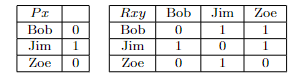
\includegraphics{Pictures/Week8.png}

Evaluate the following formulas for truth or falsity:

\begin{enumerate}
\def\labelenumi{\arabic{enumi}.}
\tightlist
\item
  \(Pb\)
\item
  \(Rbz\)
\item
  \((Pb \lor Rbz)\)
\item
  \(((\sim Pb \& Rbz) \equiv Rjz)\)
\item
  \(\sim (Pj \supset Rzz)\)
\item
  \(((Pb \lor Pj) \supset (Rbj \& Rzj))\)
\item
  \((Pj \supset (Rbb \supset Rjj))\)
\item
  \(\exists x(Px \& \exists y (Rxy))\)
\item
  \(\forall x \sim (Rxx)\)
\item
  \(\forall x (Px \supset Rxz)\)
\end{enumerate}

\hypertarget{solutions-3}{%
\section{Solutions}\label{solutions-3}}

Part A:

\begin{enumerate}
\def\labelenumi{\arabic{enumi}.}
\tightlist
\item
  \((Pdk \& Skd)\)
\item
  \((\sim Skd \& Fk)\)
\item
  \((Pkd \supset (Mk \lor Fk))\)
\item
  \(\forall x(Mx \supset \exists y (Pxy))\)
\item
  \(\forall x\exists y (Sxy \& Fy)\)
\item
  \(\exists x(Mx \& \sim Fx)\)
\item
  \(\forall x(Sxd \supset Fx)\)
\item
  \(\forall x(Sxd \supset \exists y(Pyx \& My))\)
\item
  \(\exists x(Pxk \& \sim(Mx \lor Fx))\)
\item
  \((Mk \& (\exists x (Sxk \supset Fx))\)
\end{enumerate}

Part B:

\begin{enumerate}
\def\labelenumi{\arabic{enumi}.}
\tightlist
\item
  \((Za \& Zb \& Zc)\)
\item
  \((Rb \& \sim Gb)\)
\item
  \((Lcb \supset Mb)\)
\item
  \(((Gb \& Gc) \supset (Lab \& Lac))\)
\item
  \(\forall x((Ax \& Zx) \supset (Mx \lor Gx))\)
\item
  \(\exists x(Rx \& Zx)\)
\item
  \(\forall x(Gx \supset Rx)\)
\item
  \(\exists x(Rx \& \sim Gx)\)
\item
  \(\forall x((Mx \& Zx) \supset Lbx)\)
\item
  \(\forall x((Mx \& Lcx) \supset Lax)\)
\end{enumerate}

Part C:

\begin{enumerate}
\def\labelenumi{\arabic{enumi}.}
\tightlist
\item
  New York is north of and east of Los Angeles.
\item
  Hong Kong is not north of Paris and Paris is not east of New York.
\item
  All metropolises are north of Antarctica.
\item
  There is a town north of New York.
\item
  Everything is a town east of London.
\item
  New York is north of some metropolis.
\item
  All metropolises are either north of Paris or to the east of Paris.
\item
  New York is east of everything north of every town.
\item
  There is a metropolis such that all towns are not north of that metropolis.
\end{enumerate}

Part D:

\begin{enumerate}
\def\labelenumi{\arabic{enumi}.}
\tightlist
\item
  False
\item
  True
\item
  True
\item
  True
\item
  True
\item
  True
\item
  True
\item
  True
\item
  True
\item
  True
\end{enumerate}

  \bibliography{book.bib,packages.bib}

\end{document}
